\section{緒言}

\subsection{研究背景}

一般的に,流体はせん断応力がせん断速度に比例するNewton流体と,せん断応力がせん断速度が非線形となる非Newton流体に分類することができる.様々な流体のせん断速度とせん断応力の関係をFig\ref{fig:1-fluid-curve}(a)に示す\cite{ref:1}.Newton流体はせん断速度とせん断応力が比例関係にある流体である.一方でそれ以外の流体は非Newton流体と呼ばれている.非Newton流体は Shear thinning 流体(Pseudoplastic), Shear thickening 流体(Dilatant fluid), Bingham plastic 流体, Viscoplastic 流体, Viscoelastic 流体が挙げられている.非Newton流体のうち,Bingham plastic 流体, Viscoplastic 流体はせん断応力がある一定になるまでせん断速度が発生しない流体である.これらの一例として,バターや冷却途中の溶岩などが挙げられる\cite{mendes2004viscosity,balmforth2000visco}.一方で,Shear-thinning 流体, Shear-thinning 流体はせん断応力が少しでも加わると,せん断速度が発生し流体的挙動を示す.Shear-thinning 流体の一例として,マヨネーズや血液,泥,ポリマーなどが挙げられる\cite{liu2007rheological,bodnar2011shear,hu2017shear,ryder2006shear}.Shear-thickening 流体の一例として,水溶き片栗粉や液体ボディアーマー,ブレーキパッドなどが挙げられる\cite{crawford2013shear,haris2017effectiveness,zarei2020application}.また,Viscoelastic 流体は粘性だけでなく弾性的挙動を示す流体である.この一例として流動ゴムや高分子融体が挙げられる\cite{stieger2021influence,boger1987viscoelastic}.

非Newton流体の粘度を示すモデルとして,Power-law model (Ostwald-De Waele model)\cite{Ostwald1929}, Cross model\cite{cross1965rheology}, Carreau model\cite{carreau1972rheological}, Carreau-Yasuda model\cite{yasuda1979investigation}やHerschel-Bulkley model\cite{briscoe1994properties,de1998fresh}などを挙げることができる\cite{ref:1}.Power-law model はせん断速度の限られた範囲内にて適応することができる.Cross modelはshear-thinning性が構造的に引き起こされるといった仮説において導き出されたモデルである.これは広いせん断速度において適用することができる.また,Carreau model はCross modelをPower-law領域においてより適合するよう修正したものとなっている.Carreau-Yasuda model は,Carreau model を粘度減少が開始する特性時間に関してより適合するように修正されたものである.Herschel-Bulkley modelはBingham plasticやViscoplasticといった静止状態の流体においてせん断応力が存在する流体を示すモデルとなっている\cite{ref:1}.

Power-lawモデル式中の指数によってNewton流体,Shear-thinning流体と,Shear-thickening流体に分類することができる.これらのせん断速度と粘度の関係性をFig\ref{fig:1-fluid-curve}(b)に示す.これら2種類の流体のうち,本研究で扱うShear-thinning流体は,せん断速度$\dot{\gamma}$が高くなるほど粘度$\mu$が低くなる性質を有している.この流体は擬塑性流体とも呼ばれている.産業分野において,擬塑性流体の輸送を行うことがある.少ないエネルギーで輸送を行うためには,せん断速度が高くなるほど粘度が低くなる性質を活かし,抵抗低減を図る必要がある.

流体中を運動する気泡や剛体周囲流体の粘度分布や流動構造から,その運動に対する影響を明らかにする必要があり,様々な研究が行われてきた.例えば,Ohta \textit{et al}. \cite{ref:2}は非弾性擬塑性流体中における液滴の上昇運動に対し,液滴周りのせん断速度による粘度低下があたえる影響を明らかにした.加えて,Ohta \textit{et al}. \cite{ref:3}は液滴周りの粘度分布を数値計算より求め,局所的な粘度低下は液滴の形状に大きく依存することを明らかにした.また,Zhang \textit{et al}. \cite{ref:4}は非弾性擬塑性流体中における単一気泡の上昇運動に対し,後方に生じる2つの高粘度領域が気泡の上昇運動に影響を与えることを明らかにした.

超音波振動の影響による抵抗低下の一例として,van den Wildenberg \textit{et al}.\cite{ref:6}による研究があげられる.彼らの研究では,粒子の上部を水で満たした容器ごと振動させ,その粒子中に球を落下させた.その結果をFig\ref{fig:4-sinking}に示す.
(a)は球の落下時間と落下球の位置の関係を表し,(b)は落下球の位置と落下速度の関係を表す.1は,落下球の半径が4mm,2は,落下球の半径が7mmである.Fig\ref{fig:4-sinking}(a)において,$\Gamma$は振動強度である.振動によって落下球表面におけるせん断応力が減少し,振動強度を強くするとより深くまで沈降すると報告された.Iwata \textit{et al}.\cite{ref:5}は,擬塑性流体中における気泡の体積を超音波振動によって周期的に増加・減少させた.気泡の膨張収縮に伴い,周囲流体が変形し粘度低下を発生させた.周囲流体の粘度低下により,上昇速度が増加することを明らかにした.

本研究において試験溶液としたポリマーの流動は,粘性だけでなく弾性にも依存する\cite{viscoelasticity}.ポリマーの動的粘弾性特性に関する研究として,Tanaka \textit{et al}.\cite{田中勝敏1993ポリアミド}が挙げられる.彼らの研究では,ポリアミドとポリプロピレンのポリマーブレンドを行い動的粘弾性計測を行った.混合後のポリマーと母材であるポリアミド,ポリプロピレンの動的粘弾性特性の比較を行い,母材による影響を明らかにした.

また,岩室\cite{ref:8}は擬塑性流体中を落下する球に超音波振動を照射し,流体物性,物体形状,超音波強度および周波数を変化させることで調査を行った.この場合,落下速度の高速化は音響境界層内部における粘度低下と,音響境界層の形成が関係していると明らかにした.落下球の球径を変化させた場合,落下球によって生じる周囲流体の応力が変化する.周囲流体に生じる応力が変化することで,粘性影響だけでなく弾性影響が生じることも示された.また,弾性影響により高速化が抑制されることが示唆された.しかし,調査された流体物性は限定的であり,弾性影響による高速化の抑制は十分に議論されていない.
\begin{figure}[ht]
    \centering
    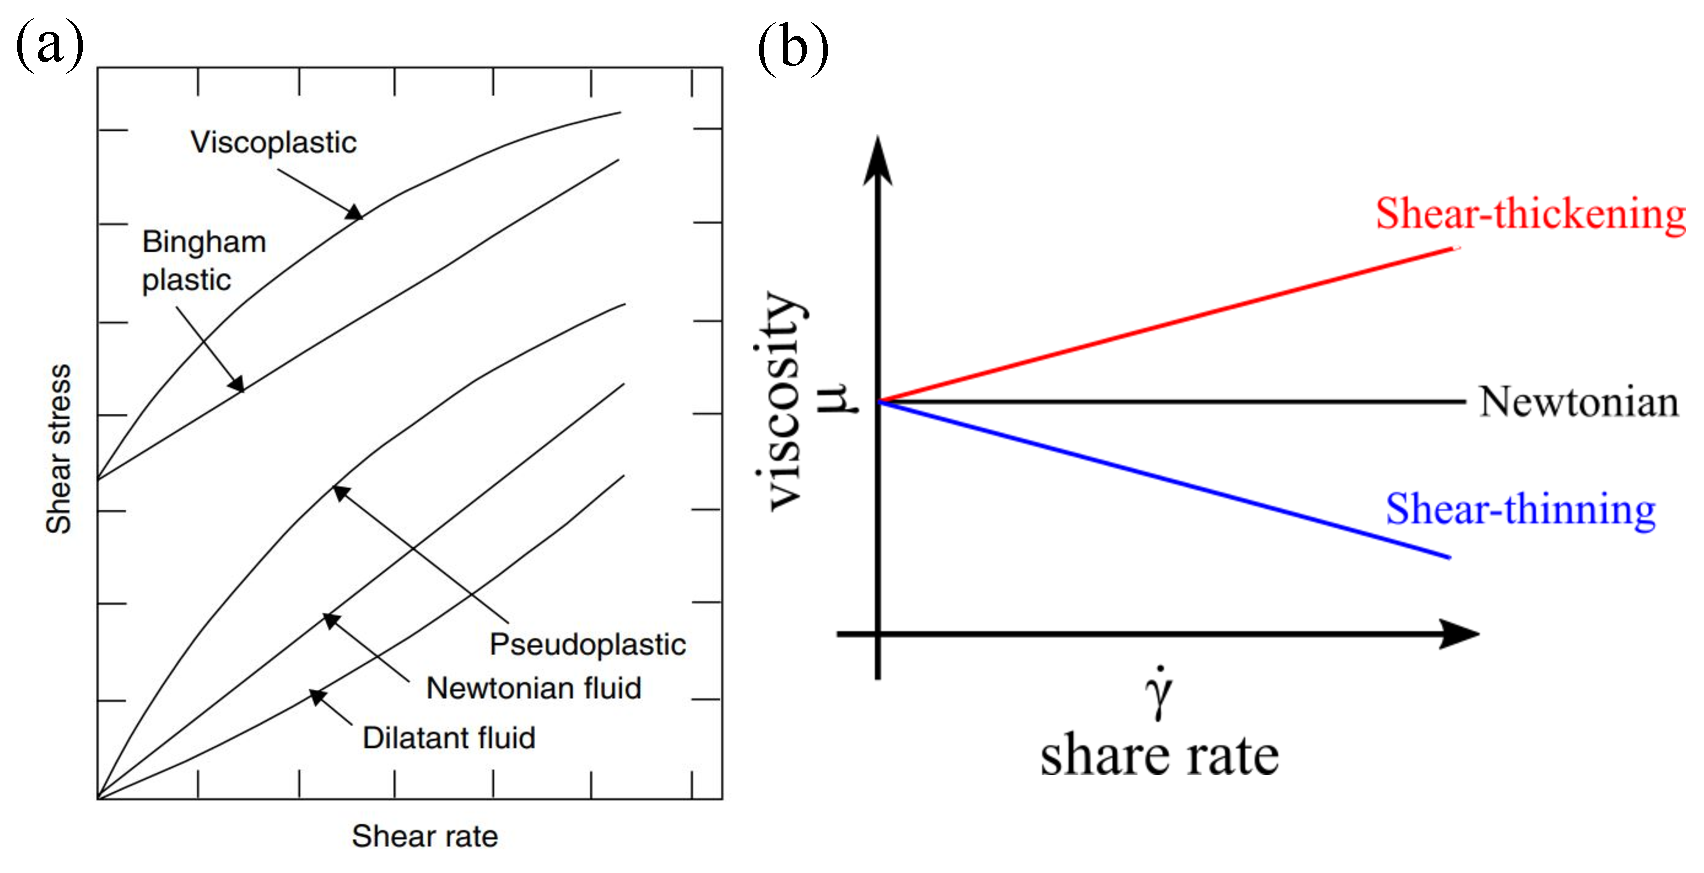
\includegraphics[width=1\textwidth]{1-Background/shea-thining.eps}
    \caption{(a) Qualitative flow curves for different types of non-Newtonian fluids\cite{ref:1}. (b)Classifications of non-Newtonian power-law fluid.}
    \label{fig:1-fluid-curve}
\end{figure}
\begin{figure}[ht]
    \begin{center}
        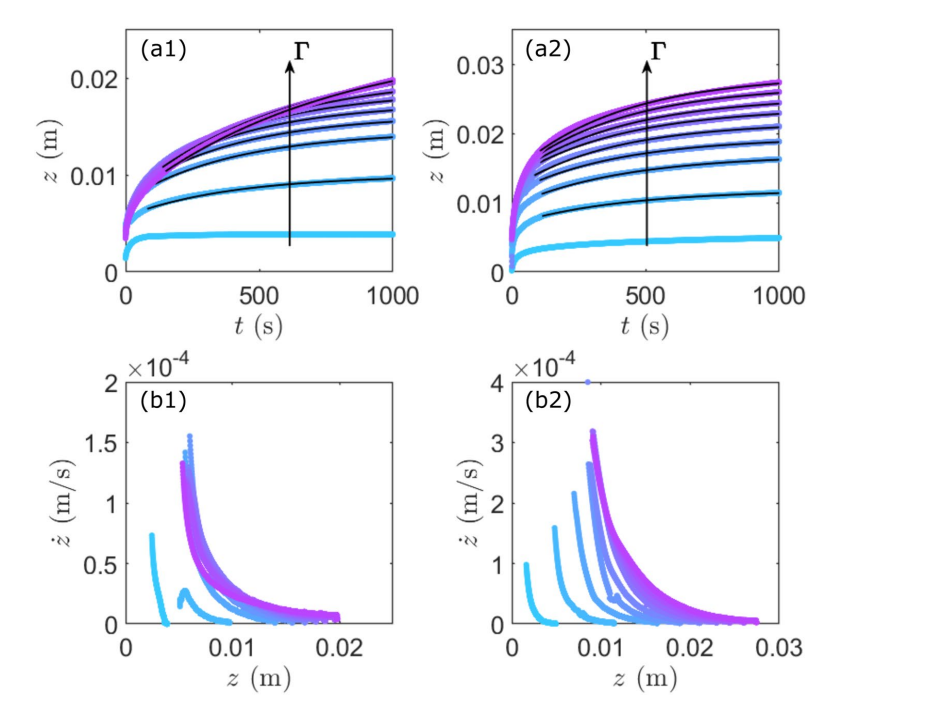
\includegraphics[width=12.0cm,clip]{1-Background/4-sinking.png}
        \caption{Sinking dynamics for different intruder-sizes and for different vibration intensities $\Gamma$. (a1) Depth$z$ versus time$t$ for $\dot{z}$ an intruder with radius of 4mm and (a2) for an intruder with radius of 7mm. (b1) Instantaneous velocity versus sinking depth $z$ obtained from (a1) and (b2) from (a2). The black lines correspond to the solutions fitted in the quasi-steady regime\cite{ref:6}.}
        \label{fig:4-sinking}
    \end{center}
\end{figure}
\newpage
\subsection{研究目的}

先行研究\cite{ref:8}において,超音波照射された擬塑性流体中を落下する球の高速化の要因として,音響境界層内部における粘度低下と,音響境界層の形成が関係していることが明らかにされている.また,高速化が弾性によって抑制されることを示唆していた.しかし,調査された流体や落下球の種類,径は限定的であり,弾性が高速化抑制することを明らかにしていない.落下球の密度や濃度密度を大きく変化させることで,球の周囲に生じる応力を変化させ,粘性と弾性それぞれ影響を明らかにすることができる.

本研究で用いた試験溶液では,球の落下による運動が高速の場合,粘性による影響が支配的であり,低速の場合は弾性による影響が支配的となる.落下球の終端速度を変化させることで粘性が支配的な場合と弾性が支配的な場合に分けて,超音波照射による高速化への影響を調査した.そこで,流体物性,落下物体の密度,落下球の径をより大きく変化させ実験を行った.超音波照射された擬塑性流体中を落下する球の高速化に対する粘弾性両方の影響を明らかにすることを目的とする.
